\section{Introduction}

\sectioncover

\subsection{Background}

\begin{frame}
  \begin{itemize}
    \item<1-> Fracture is a common phenomenon in engineering applications.
    
    \item<2-> To characterize fracture by its \textbf{consequence}: \textcolor<3>{red}{fragmentation}, \textcolor<4>{red}{desiccation}, \textcolor<5>{red}{ductile failure}, \textcolor<6>{red}{spallation}, etc.. \\
    \only<3-6>{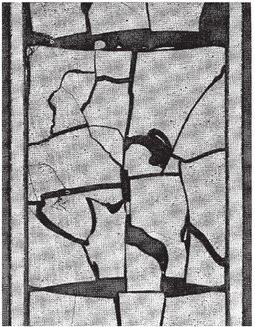
\includegraphics[width=0.12\textwidth]{Chapter1/figures/fragmentation}}
    \only<4-6>{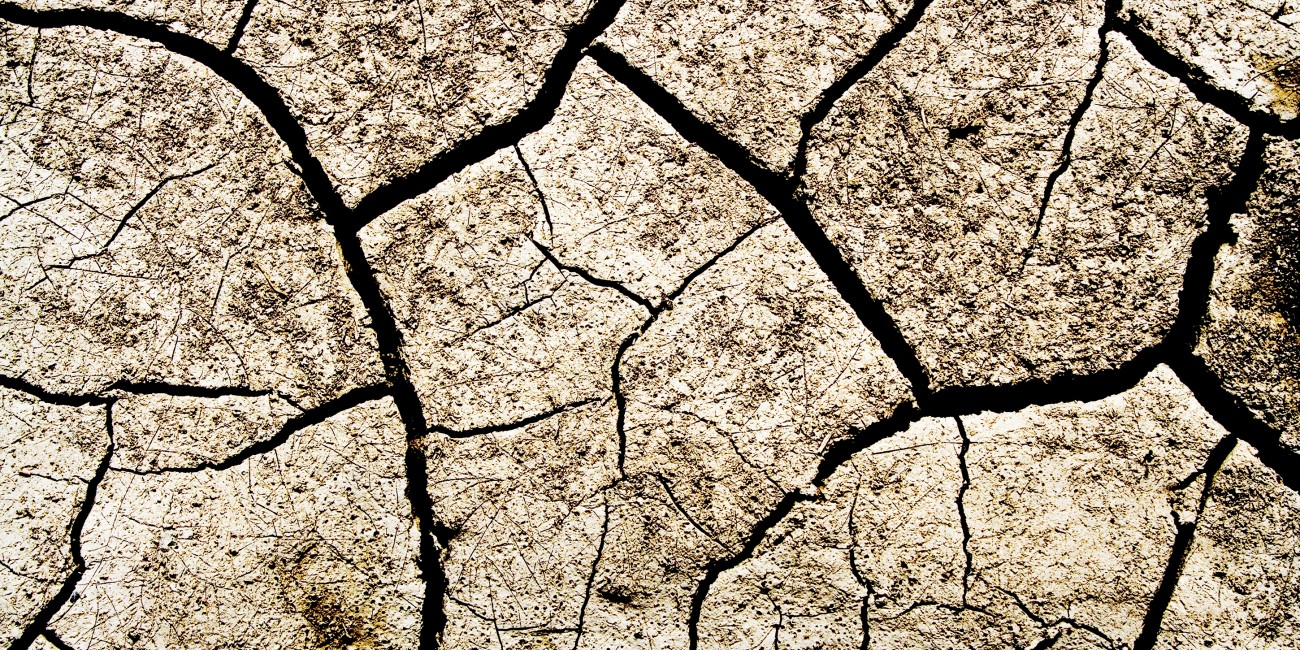
\includegraphics[width=0.3\textwidth]{Chapter1/figures/desiccation}}
    \only<5-6>{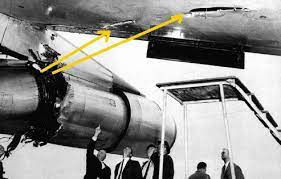
\includegraphics[width=0.24\textwidth]{Chapter1/figures/ductile_failure}}
    \only<6>{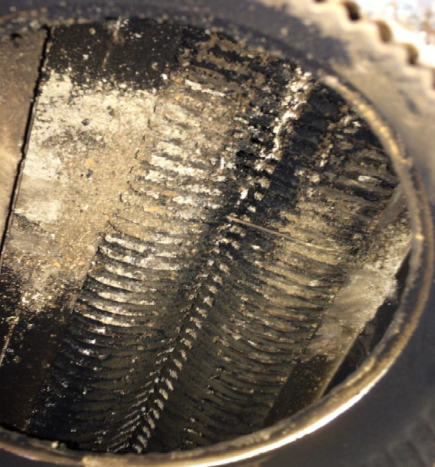
\includegraphics[width=0.14\textwidth]{Chapter1/figures/spallation}}
    
    \item<7-> To characterize fracture by its \textbf{development lifecycle}: \textcolor<8>{red}{defects, nucleation}, \textcolor<9>{red}{propagation}, \textcolor<10>{red}{branching}, \textcolor<11>{red}{merging}. \\
    \only<8>{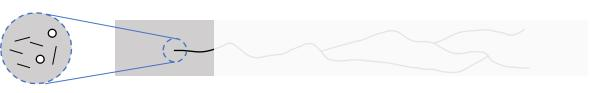
\includegraphics[width=0.75\textwidth]{Chapter1/figures/nucleation}}
    \only<9>{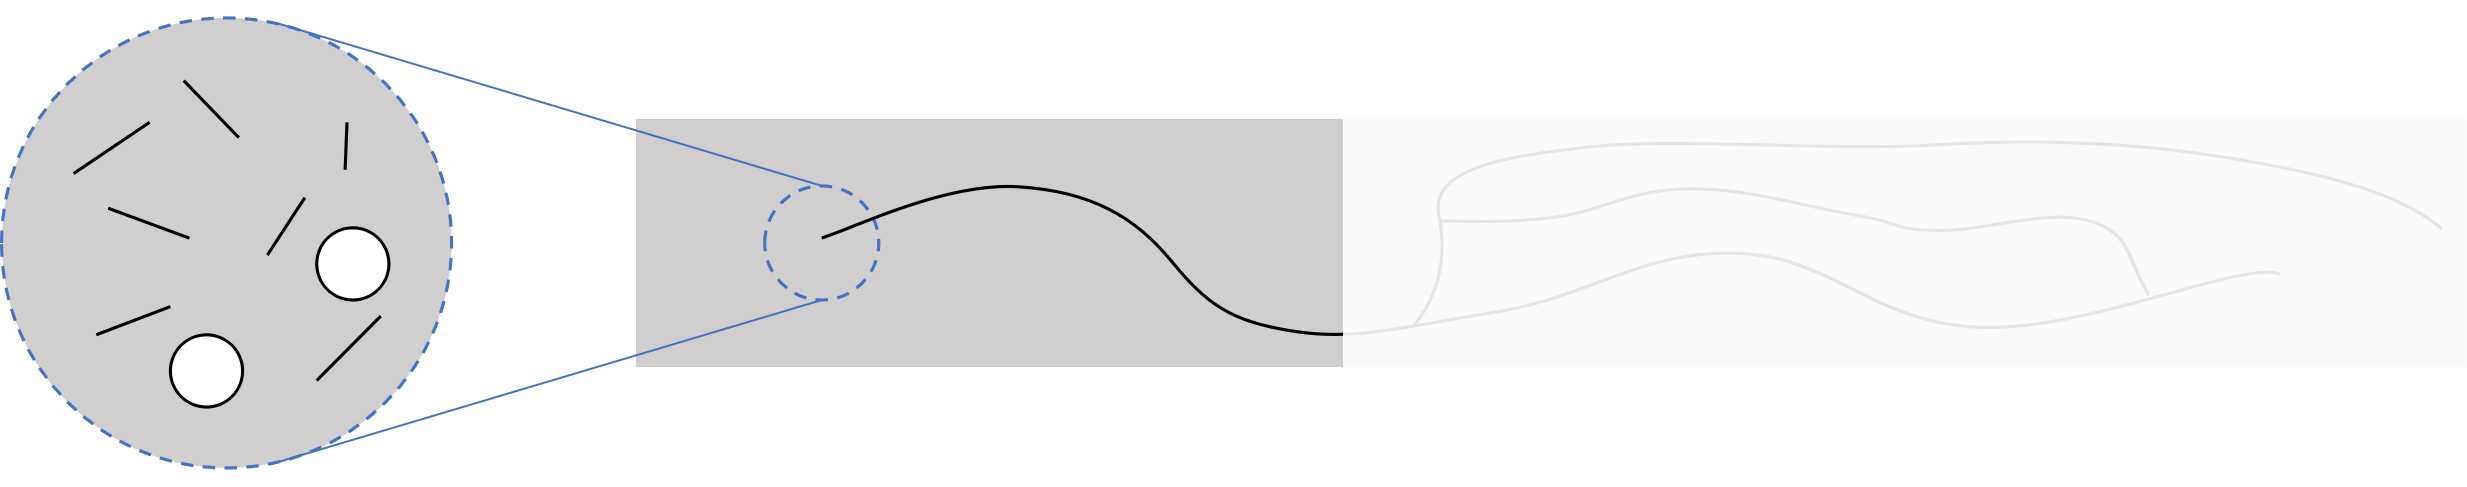
\includegraphics[width=0.75\textwidth]{Chapter1/figures/propagation}}
    \only<10>{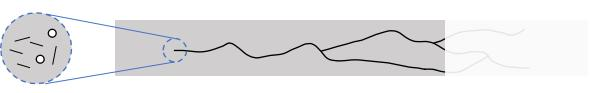
\includegraphics[width=0.75\textwidth]{Chapter1/figures/branching}}
    \only<11>{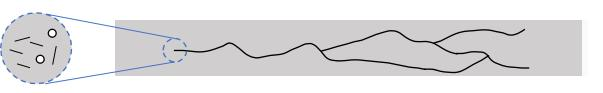
\includegraphics[width=0.75\textwidth]{Chapter1/figures/merging}}
    
    \item<12-> To categorize fracture by \textbf{material response}:
    \begin{itemize}
      \item<13-> brittle fracture: singularities, abrupt failure, tiny fracture process zone;
      \item<14-> quasi-brittle fracture: softening, small fracture process zone;
      \item<15-> cohesive fracture: softening, large fracture process zone;
      \item<16-> ductile fracture: plastic deformation prior to fracture;
      \item<16-> ...
    \end{itemize}
    \only<13-16>{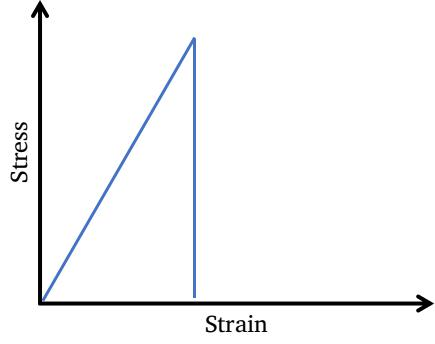
\includegraphics[width=0.2\textwidth]{Chapter1/figures/brittle}}
    \only<14-16>{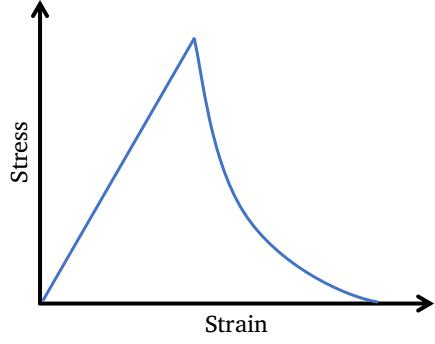
\includegraphics[width=0.2\textwidth]{Chapter1/figures/cohesive}}
    \only<16-16>{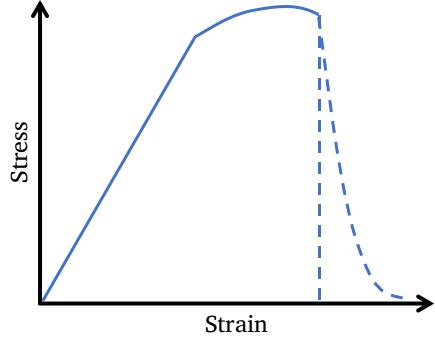
\includegraphics[width=0.2\textwidth]{Chapter1/figures/ductile}}
    
    \item<17-> Coupling with other phenomena: dynamics, viscous dissipation, thermal effects, plasticity, creep, etc..
  \end{itemize}
  
  \only<18->{
    \begin{block}{}
      \centering
      \vspace{1em}
      To date, fracture is still one of the most challenging phenomena to model and predict.
      \vspace{1em}
    \end{block}
  }
\end{frame}

\subsection{Phase-field approach to fracture}

\begin{frame}
  \vspace{-2em}
  \begin{columns}
    \begin{column}{0.75\textwidth}
      \only<1->{
        \begin{block}{}
          The permanent crack set $\Gamma$ and its associated fracture energy
          \begin{align*}
            \Psi^f = \int_\Gamma \Gc \diff{A}
          \end{align*}
        \end{block}
      }
      \only<2->{
        is approximated with
        
        \begin{block}{}
          the crack surface density function $\gamma = \widehat{\gamma_l}(d)$:
          \begin{align*}
            \Psi^f & \approx \int_\body \Gc \gamma \diff{V}, \quad \gamma = \dfrac{1}{c_0l}\left( \alpha + l^2 \grad d \cdot \grad d \right). 
          \end{align*}
          \begin{itemize}
            \item $d \in [0, 1]$ is the phase field;
            \item $\alpha = \widehat{\alpha}(d)$ is the crack geometric function, $\widehat{\alpha}(0) = 0$, $\widehat{\alpha}(1) = 1$;
            \item $g = \widehat{g}(d)$ is the degradation function, $\widehat{g}(0) = 1$, $\widehat{g}(1) = 0$;
            \item $c_0$ is chosen such that
                  \begin{align*}
                    \lim_{l \to 0^+} \int_\body \Gc \gamma \diff{V} = \int_\Gamma \Gc \diff{A}.
                  \end{align*}
          \end{itemize}
        \end{block}
        See \cite{bourdin2008variational} for more details.
      }
    \end{column}
    \begin{column}{0.25\textwidth}
      \only<1->{
        \begin{figure}
          \centering
          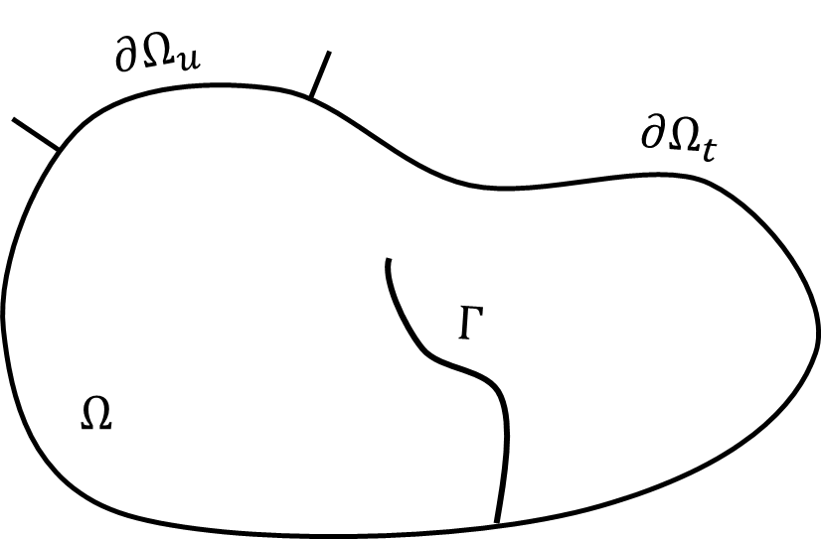
\includegraphics[width=\textwidth]{Chapter1/figures/potato_broken}
        \end{figure}
      }
      \only<2->{
        \begin{figure}
          \centering
          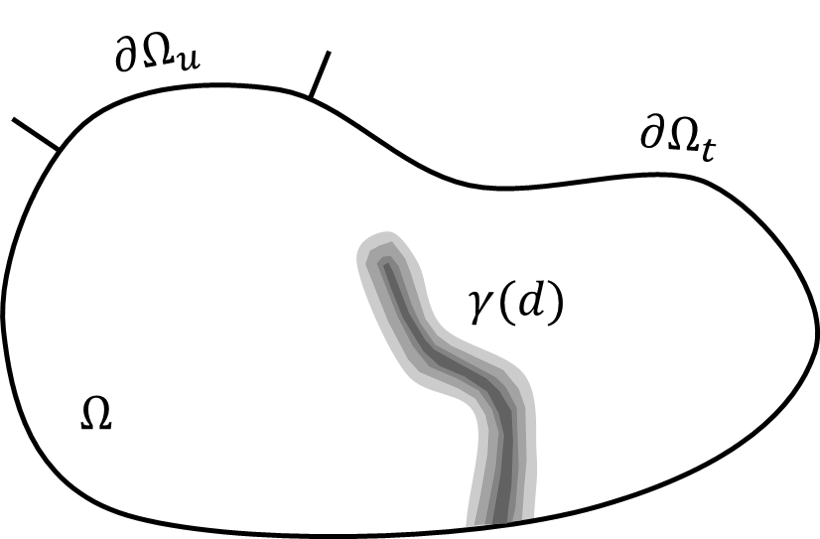
\includegraphics[width=\textwidth]{Chapter1/figures/potato_diffuse}
        \end{figure}
      }
    \end{column}
  \end{columns}
\end{frame}
